% Created 2014-10-09 星期四 10:41
\documentclass{article}
\usepackage{fixltx2e}
\usepackage{graphicx}
\usepackage{longtable}
\usepackage{float}
\usepackage{wrapfig}
%\usepackage{soul}
%\usepackage{textcomp}
%\usepackage{marvosym}
%\usepackage{wasysym}
%\usepackage{latexsym}
%\usepackage{amssymb}
\usepackage{hyperref}
\tolerance=1000
\usepackage{etex}
\usepackage{amsmath}
\usepackage{pstricks}
\usepackage{pgfplots}
\usepackage{tikz}
\usepackage[europeanresistors,americaninductors]{circuitikz}
\usepackage{colortbl}
\usepackage{yfonts}
\usetikzlibrary{shapes,arrows}
\usetikzlibrary{positioning}
\usetikzlibrary{arrows,shapes}
\usetikzlibrary{intersections}
\usetikzlibrary{calc,patterns,decorations.pathmorphing,decorations.markings}
\usepackage[BoldFont,SlantFont,CJKchecksingle]{xeCJK}
\setCJKmainfont[BoldFont=Evermore Hei]{Evermore Kai}
\setCJKmonofont{Evermore Kai}
\usepackage{pst-node}
\usepackage{pst-plot}
\psset{unit=5mm}
\usepackage{beamerarticle}
\mode<beamer>{\usetheme{Frankfurt}}
\mode<beamer>{\usecolortheme{dove}}
\mode<article>{\hypersetup{colorlinks=true,pdfborder={0 0 0}}}
\AtBeginSection[]{\begin{frame}<beamer>\frametitle{Topic}\tableofcontents[currentsection]\end{frame}}
\setbeamercovered{transparent}
\providecommand{\alert}[1]{\textbf{#1}}

\title{自动控制的基本概念}
\author{}
\date{}
\hypersetup{
  pdfkeywords={},
  pdfsubject={},
  pdfcreator={Emacs Org-mode version 7.9.3f}}

\begin{document}

\maketitle

\begin{frame}
\frametitle{Outline}
\setcounter{tocdepth}{3}
\tableofcontents
\end{frame}










\section{自动控制历史}
\label{sec-1}
\subsection{自动控制历史}
\label{sec-1-1}
\begin{frame}
\frametitle{Centrifugal governor}
\label{sec-1-1-1}

\includegraphics[width=\textwidth]{image/centrifugal_governor.png}
\end{frame}
\begin{frame}
\frametitle{Tolilet Valve}
\label{sec-1-1-2}

\includegraphics[width=\textwidth]{image/250px-Gravity_toilet_valves_handle_down.svg.png}
\end{frame}
\begin{frame}
\frametitle{指南车}
\label{sec-1-1-3}

\includegraphics[width=\textwidth]{image/zhinanche.jpg}
\end{frame}
\begin{frame}
\frametitle{莲花漏}
\label{sec-1-1-4}

\includegraphics[width=\textwidth]{image/lianhualou.jpg}
\end{frame}
\begin{frame}
\frametitle{Windmil fantail}
\label{sec-1-1-5}

\includegraphics[height=\textheight]{image/DK_Fanoe_Windmill01.JPG}
\end{frame}
\begin{frame}
\frametitle{telautograph}
\label{sec-1-1-6}

\includegraphics[width=\textwidth]{image/telautograph.jpg}
\end{frame}
\begin{frame}
\frametitle{控制理论的发展}
\label{sec-1-1-7}

\begin{itemize}
\item <1> Pierre-Simon Laplace (1749-1827) invented the Z-transform in his work on probability theory, now used to solve discrete-time control theory problems. The Z-transform is a discrete-time equivalent of the Laplace transform which is named after him.
\item <2> Joseph Fourier (21 March 1768 – 16 May 1830) was a French mathematician and physicist born in Auxerre and best known for initiating the investigation of Fourier series and their applications to problems of heat transfer and vibrations. The Fourier transform and Fourier's Law are also named in his honour. Fourier is also generally credited with the discovery of the greenhouse effect.
\item <3> James Clerk Maxwell (13 June 1831 – 5 November 1879) published a paper On governors in the Proceedings of Royal Society, vol. 16 (1867–1868). This paper is considered a central paper of the early days of control theory. Here ``governors'' refers to the governor or the centrifugal governor used to regulate steam engines.
\end{itemize}
\end{frame}
\begin{frame}
\frametitle{控制理论的发展}
\label{sec-1-1-8}

\begin{itemize}
\item <1> Alexander Lyapunov (1857–1918) in the 1890s marks the beginning of stability theory.
\item <2> Harold S. Black (1898–1983), invented the concept of negative feedback amplifiers in 1927. He managed to develop stable negative feedback amplifiers in the 1930s.
\item <3> Norbert Wiener (1894–1964) co-developed the Wiener–Kolmogorov filter and coined the term cybernetics in the 1940s.
\end{itemize}
\end{frame}
\begin{frame}
\frametitle{控制理论的发展}
\label{sec-1-1-9}

\begin{itemize}
\item <1> Harry Nyquist (1889–1976), developed the Nyquist stability criterion for feedback systems in the 1930s.
\item <2> Claude Elwood Shannon (April 30, 1916 – February 24, 2001) is also credited with the introduction of sampling theory, which is concerned with representing a continuous-time signal from a (uniform) discrete set of samples.
\end{itemize}
\begin{itemize}
\item <3> Hendrik Wade Bode (pronounced Boh-dee in English, Boh-dah in Dutch),(24 December 1905 – 21 June 1982) was an American engineer, researcher, inventor, author and scientist, of Dutch ancestry.
      He made important contributions to control system theory and mathematical tools for the analysis of stability of linear systems, inventing Bode plots, gain margin and phase margin.
\end{itemize}
\end{frame}
\begin{frame}
\frametitle{控制理论的发展}
\label{sec-1-1-10}

\begin{itemize}
\item <1> John R. Ragazzini (1912–1988) introduced digital control and the use of Z-transform in control theory (invented by Laplace) in the 1950s.
\item <2> Walter Richard Evans (January 15, 1920 - July 10, 1999) was a noted American control theorist and the inventor of the root locus method in 1948.
\item <3> In control systems theory, the describing function (DF) method, developed by Nikolay Mitrofanovich Krylov and Nikolay Bogoliubov in the 1930s, and extended by Ralph Kochenburger is an approximate procedure for analyzing certain nonlinear control problems.
\end{itemize}
\end{frame}
\subsection{自动控制理论}
\label{sec-1-2}
\begin{frame}
\frametitle{自动控制}
\label{sec-1-2-1}

 无人工直接参与的情况下,利用控制装置(控制器)使被控对象按照给定的规律变化。
\end{frame}
\begin{frame}
\frametitle{自动控制理论}
\label{sec-1-2-2}

\begin{itemize}
\item <2->经典控制理论
\item <3->现代控制理论
\end{itemize}
\end{frame}
\begin{frame}
\frametitle{课程内容:}
\label{sec-1-2-3}

\begin{enumerate}
\item <2->一般概念
\item <3->数学模型
\item <4->分析方法
\begin{enumerate}
\item 时域分析法
\item 根轨迹法
\item 频域分析法
\end{enumerate}
\item <5->设计方法
\item <6->离散系统分析
\item <7->典型非线性系统的分析
\end{enumerate}
\end{frame}
\section{反馈与控制}
\label{sec-2}
\subsection{开环控制}
\label{sec-2-1}
\begin{frame}
\frametitle{开环控制}
\label{sec-2-1-1}

\begin{itemize}
\item <2->定义:开环控制是指控制器与被控对象之间只有顺向作用而没有反向联系,称为开环控制。
\item <3->系统的输出量对系统的输入量无影响
\item <4->开环系统对控制偏差无修正能力。
\begin{itemize}
\item <5->按给定量控制
\item <6->按扰动量控制
\end{itemize}
\end{itemize}
\end{frame}
\begin{frame}
\frametitle{按给定量控制}
\label{sec-2-1-2}



\begin{tikzpicture}[node distance=2em,auto,>=latex', thick]
%\path[use as bounding box] (-1,0) rectangle (10,-2); 
\path[->] node[] (r) {$U_g$}; 
%\path[->] node[ circle,inner sep=2pt,minimum size=1pt,draw,label=below left:$ $,right =of r] (p1) { }; 
%\path[->](r) edge node {} (p1) ; 
\path[blue] node[draw, right =of r] (n) {信号变换与驱动电路}; 
\path[->] (r) edge node[midway] {} (n) ; 
\path[red] node[draw, inner sep=5pt,right =of n] (g) {电机}; 
\path[->] (n) edge node [midway]{$ $} (g); 
\path[->] node[ right =of g] (o) {$n$}; 
\path[->] (g) edge node {} (o); 
%\path[blue] node[draw, below =of g] (h) {传感器};
%\path[->,draw] (g.east)+(1em,0) |- (h.east) ; 
%\path[->,draw] (h.west) -| (p1) ; 
\end{tikzpicture} 

\begin{itemize}
\item 输入量: 电压 $U_g$
\item 输出量: 电机转速 $n$
\item $n=kU_g$
\end{itemize}
\end{frame}
\begin{frame}
\frametitle{按扰动量控制}
\label{sec-2-1-3}

   对扰动进行补偿,使扰动的影响减小


\begin{tikzpicture}[node distance=2em,auto,>=latex', thick]
%\path[use as bounding box] (-1,0) rectangle (10,-2); 
\path[->] node[] (r) {$U_0$}; 
\path[->] node[ circle,inner sep=2pt,minimum size=1pt,draw,label=below left:$ $,right =of r] (p1) { }; 
\path[->](r) edge node {} (p1) ; 
\path[blue] node[draw, right =of p1] (n) {驱动电路}; 
\path[->] (p1) edge node[midway] {$U_c$} (n) ; 
\path[red] node[draw, inner sep=5pt,right =of n] (g) {电机}; 
\path[->] (n) edge node [midway]{$ $} (g); 
\path[->] node[ right =of g] (o) {$n$}; 
\path[->] (g) edge node {} (o); 
\path[blue] node[draw, below =of g] (l) {负载扰动};
\path[dashed,draw] (g.south) edge (l) ; 
\path[blue] node[draw, below =of n] (h) {扰动测量};
\path[->,draw] (l) edge  node[midway] {$i$} (h) ; 
\path[->,draw] (h.west) -| node[midway]{$U_b$} (p1) ; 
\end{tikzpicture} 

\begin{itemize}
\item $U_c=U_0+U_b$
\item 负载增加导致 $n\downarrow , i\uparrow$
\item $i\uparrow\rightarrow U_b\uparrow\rightarrow U_c\uparrow\rightarrow n\uparrow$
\end{itemize}
\end{frame}
\begin{frame}
\frametitle{开环控制特点}
\label{sec-2-1-4}

\begin{enumerate}
\item <2->优点:原理简单,结构简单,反应速度快,灵敏度高
\item <3->缺点:
\begin{itemize}
\item 对控制偏差无修正能力
\item 控制精度取决于各控制元器件的精度
\end{itemize}
\item <4->适应场合:对控制精度要求不高的系统
\item <5-> 结构图:   输入 $\rightarrow$ 控制器 $\rightarrow$ 被控对象 $\rightarrow$ 输出  (顺向作用)
\end{enumerate}
\end{frame}
\subsection{闭环控制}
\label{sec-2-2}
\begin{frame}
\frametitle{闭环控制}
\label{sec-2-2-1}


\begin{tikzpicture}[node distance=2em,auto,>=latex', thick]
%\path[use as bounding box] (-1,0) rectangle (10,-2); 
\path[->] node[] (r) {期望}; 
\path[->] node[ circle,inner sep=2pt,minimum size=1pt,draw,label=below left:$ $,right =of r] (p1) { }; 
\path[->](r) edge node {} (p1) ; 
\path[blue] node[draw, right =of p1] (n) {控制器}; 
\path[->] (p1) edge node[midway] {偏差} (n) ; 
\path[red] node[draw, inner sep=5pt,right =of n] (g) {被控对象}; 
\path[->] (n) edge node [midway]{$ $} (g); 
\path[->] node[ right =of g] (o) {输出}; 
\path[->] (g) edge node {} (o); 
\path[blue] node[draw, below =of g] (h) {传感器};
\path[->,draw] (g.east)+(1em,0) |- (h.east) ; 
\path[->,draw] (h.west) -| (p1) ; 
\end{tikzpicture} 

\begin{itemize}
\item <2-> 定义: 闭环控制是指在输出量处,通过 \textbf{反馈} 回路使得输出量对输入量施加影响
\item <3-> 控制目的:通过在输入端引入输出量,使得输入处的偏差 $\rightarrow0$
\item <4->闭环控制按偏差进行调节。
\end{itemize}
\end{frame}
\begin{frame}
\frametitle{反馈}
\label{sec-2-2-2}

\begin{itemize}
\item 反馈: 指将系统的输出返回到输入端并以某种方式改变输入,进而影响系统功能的过程。
\item 正反馈: 输出变化时,反馈对输出造成的影响与输出变化趋势相同
\item 负反馈:输出变化时,反馈对输出造成的影响与输出变化趋势相反
\end{itemize}
\end{frame}
\begin{frame}
\frametitle{示例:人手工竖杆}
\label{sec-2-2-3}
\begin{itemize}

\item 示意图\\
\label{sec-2-2-3-1}%
%LaTeX with PSTricks extensions
%%Creator: 0.48.2
%%Please note this file requires PSTricks extensions
\psset{xunit=.5pt,yunit=.5pt,runit=.5pt}
\begin{pspicture}(83.9397583,146.67623901)
{
\newrgbcolor{curcolor}{0 0 0}
\pscustom[linewidth=1,linecolor=curcolor]
{
\newpath
\moveto(77.59144242,73.33811721)
\curveto(77.59144242,66.87824605)(71.75959493,61.64148578)(64.56564648,61.64148578)
\curveto(57.37169803,61.64148578)(51.53985055,66.87824605)(51.53985055,73.33811721)
\curveto(51.53985055,79.79798837)(57.37169803,85.03474864)(64.56564648,85.03474864)
\curveto(71.75959493,85.03474864)(77.59144242,79.79798837)(77.59144242,73.33811721)
\closepath
}
}
{
\newrgbcolor{curcolor}{0 0 0}
\pscustom[linewidth=1,linecolor=curcolor]
{
\newpath
\moveto(63.7681501,61.64148901)
\lineto(64.2998101,25.48826201)
\lineto(39.3115501,0.49999901)
}
}
{
\newrgbcolor{curcolor}{0 0 0}
\pscustom[linewidth=1,linecolor=curcolor]
{
\newpath
\moveto(64.2998101,24.95659701)
\lineto(80.7814301,4.75332301)
}
}
{
\newrgbcolor{curcolor}{0 0 0}
\pscustom[linewidth=1,linecolor=curcolor]
{
\newpath
\moveto(83.4397601,36.65322901)
\lineto(64.2998101,49.41319201)
\lineto(36.1215601,36.12156401)
\lineto(0.5000001,146.17624001)
}
}
\end{pspicture}



\item 分析
\label{sec-2-2-3-2}%
\begin{tikzpicture}[node distance=2em,auto,>=latex', thick]
%\path[use as bounding box] (-1,0) rectangle (10,-2); 
\path[->] node[] (r) {0}; 
\path[->] node[ circle,inner sep=2pt,minimum size=1pt,draw,label=below left:$ $,right =of r] (p1) { }; 
\path[->](r) edge node {} (p1) ; 
\path[blue] node[draw, right =of p1] (n) {脑}; 
\path[->] (p1) edge node[midway] {偏差} (n) ; 
\path[blue] node[draw, right =of n] (d) {手}; 
\path[->] (n) edge node[midway] {} (d) ; 
\path[red] node[draw, inner sep=5pt,right =of d] (g) {杆}; 
\path[->] (d) edge node [midway]{$ $} (g); 
\path[->] node[ right =of g] (o) {$\theta$}; 
\path[->] (g) edge node {} (o); 
\path[blue] node[draw, below =of d] (h) {眼};
\path[->,draw] (g.east)+(1em,0) |- (h.east) ; 
\path[->,draw] (h.west) -| (p1) ; 
\end{tikzpicture} 


\begin{itemize}
\item 反馈通道:眼
\item 执行机构:手
\item 被控制量:杆与竖直方向夹角  $\theta\rightarrow 0$
\end{itemize}

\end{itemize} % ends low level
\end{frame}
\begin{frame}
\frametitle{示例:倒立摆系统}
\label{sec-2-2-4}



\begin{tikzpicture}[node distance=2em,auto,>=latex', thick]
%\path[use as bounding box] (-1,0) rectangle (10,-2); 
\path[blue] node[draw, right =of n] (d) {电机}; 
\path[red] node[draw, inner sep=5pt,right =of d] (g) {小车}; 
\path[red,draw] (g.south)+(-0.7em,-0.25em) circle (0.25em) (g.south)+(0.7em,-0.25em) circle (0.25em);
\path[red,draw] (g.north)--+(60:3em);
\path[draw,dashed] (g.north)--+(90:3em);
\path[draw,dashed] (g.north)++(90:2.5em) arc (90:60:2.5em);
\path  (g.north)+(75:3em) node {$\theta$};
\path[] (d) edge node [midway]{$ $} (g); 
\path[blue] node[draw, right =of g] (h) {传感器};
\path[] (g) edge node {$\theta,r$}(h) ; 
\path[red,draw] (d.south)|-($(g.south)+(0,-0.51em)$)-| (h.south);

\path[blue] node[draw, below =of g] (n) {控制器}; 
\path[<-,draw] (d.west)--+(-1em,0) |- (n.west) ; 
\path[->,draw] (h.east)--+(1em,0) |- (n.east) ; 
\end{tikzpicture} 


\begin{itemize}
\item 执行机构:电机
\item 反馈通道:角度传感器、位置传感器
\item 被控制量: $\theta\rightarrow 0, r\rightarrow 0$
\end{itemize}
\end{frame}
\begin{frame}
\frametitle{示例:直流电机速度反馈控制系统}
\label{sec-2-2-5}



\begin{tikzpicture}[node distance=2em,auto,>=latex', thick]
%\path[use as bounding box] (-1,0) rectangle (10,-2); 
\path[->] node[] (r) {$U_g$}; 
\path[->] node[ circle,inner sep=2pt,minimum size=1pt,draw,label=below left:$ $,right =of r] (p1) { }; 
\path[->](r) edge node {} (p1) ; 
\path[blue] node[draw, right =of p1] (n) {放大器}; 
\path[->] (p1) edge node[midway] {$U_d$} (n) ; 
\path[red] node[draw, inner sep=5pt,right =of n] (d) {驱动电路}; 
\path[->] (n) edge node [midway]{$ $} (d); 
\path[red] node[draw, inner sep=5pt,right =of d] (g) {电机}; 
\path[->] (d) edge node [midway]{$ $} (g); 
\path[red] node[draw, inner sep=5pt,below =of g] (s) {测速电机};
\path[red] (g) edge node {$n$} (s); 
\path[->,draw] (s.west) -| node[near start] {$U_f$} node[very near end] {$-$} (p1) ; 
\end{tikzpicture} 

\begin{eqnarray}
  n  &=& K U_d \\
  U_d &=& U_g-U_f \\
  U_f &=& K' n
\end{eqnarray}

负载增大后: $n\downarrow\rightarrow U_f\downarrow\rightarrow U_d\uparrow\rightarrow n\uparrow$
\end{frame}
\begin{frame}
\frametitle{负反馈放大器}
\label{sec-2-2-6}

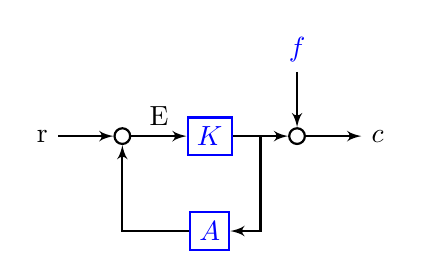
\begin{tikzpicture}[node distance=2em,auto,>=latex', thick]
%\path[use as bounding box] (-1,0) rectangle (10,-2); 
\path[->] node[] (r) {r}; 
\path[->] node[ circle,inner sep=2pt,minimum size=1pt,draw,label=below left:$ $,right =of r] (p1) { }; 
\path[->](r) edge node {} (p1) ; 
\path[blue] node[draw, right =of p1] (g) {$K$}; 
\path[->] (p1) edge node[midway] {E} (g) ; 
\path[->] node[ circle,inner sep=2pt,minimum size=1pt,draw,label=below left:$ $,right =of g] (p2) { }; 
\path[->] (g) edge node [midway]{$ $} (p2); 
\path[->] node[ right =of p2] (o) {$c$}; 
\path[->] (p2) edge node {} (o); 

\path[blue] node[draw, below =of g] (h) {$A$};
\path[->,draw] (g.east)+(1em,0) |- (h.east) ; 
\path[->,draw] (h.west) -| (p1) ; 

\path[blue] node[ above =of p2] (f) {$f$};
\path[->] (f) edge node [midway]{$ $} (p2); 
\end{tikzpicture} 

\begin{eqnarray}
c &=& Ke+f \\
e &=& r-Ac \\
c &=& \frac{Kc}{1+KA}+\frac{f}{1+KA}
\end{eqnarray}
\end{frame}
\begin{frame}
\frametitle{闭环控制的特点}
\label{sec-2-2-7}

\begin{enumerate}
\item <2->按偏差进行调节
\item <3->控制精度较高,取决于反馈通道元器件的精度,而反馈通道所包围的电路中的元器件的元件精度可降低
\item <4->抗干扰能力强
\end{enumerate}
\end{frame}
\begin{frame}
\frametitle{复合控制}
\label{sec-2-2-8}

扰动补偿+闭环控制

例:直流电机速度复合控制

\begin{tikzpicture}[node distance=2em,auto,>=latex', thick]
\tikzstyle{every node}=[font=\small]
%\path[use as bounding box] (-1,0) rectangle (10,-2); 
\path[->] node[] (r) {$U_g$}; 
\path[->] node[ circle,inner sep=2pt,minimum size=1pt,draw,label=below left:$ $,right =of r] (p1) { }; 
\path[->](r) edge node {} (p1) ; 
\path[blue] node[draw, right =of p1] (n) {放大器}; 
\path[->] (p1) edge node[midway] {$U_d$} (n) ; 
\path[->] node[ circle,inner sep=2pt,minimum size=1pt,draw,label=below left:$ $,right =of n] (p2) { }; 
\path[->](n) edge node {} (p2) ; 
\path[red] node[draw, inner sep=5pt,right =of p2] (d) {驱动电路}; 
\path[->] (p2) edge node [midway]{$ $} (d); 
\path[red] node[draw, inner sep=5pt,right =of d] (g) {电机}; 
\path[->] (d) edge node [midway]{$ $} (g); 
\path[red] node[draw, inner sep=5pt,below =of g] (s) {测速电机};
\path[red] (g) edge node {$n$} (s); 
\path[->,draw] (s.west) -| node[near start] {$U_f$} node[very near end] {$-$} (p1) ; 

\path[blue] node[draw, above =of g] (l) {负载扰动};
\path[dashed,draw] (g.north) edge (l) ; 
\path[blue] node[draw, left =of l] (h) {扰动测量};
\path[->,draw] (l) edge  node[midway] {$i$} (h) ; 
\path[->,draw] (h.west) -| node[near end]{$U_b$} (p2) ; 
\end{tikzpicture} 
\end{frame}
\section{信号与系统}
\label{sec-3}
\subsection{概念与分类}
\label{sec-3-1}
\begin{frame}
\frametitle{基本概念}
\label{sec-3-1-1}

\begin{itemize}
\item 信号: 随时间和空间变化的某种物理量.
\begin{itemize}
\item 信号通常是时间变量 $t$ 的函数
\item 信号的特性可从两方面来描述
\begin{itemize}
\item 时域特性
\item 频域特性
\end{itemize}
\end{itemize}
\item 系统: 能够对信号完成某种变换或运算功能的集合体称为系统
\end{itemize}
\end{frame}
\begin{frame}
\frametitle{闭环系统组成}
\label{sec-3-1-2}


\begin{tikzpicture}[node distance=2em,auto,>=latex', thick ]
\tikzstyle{every node}=[font=\small]
%\path[use as bounding box] (-1,0) rectangle (10,-2); 
\path[->] node[text width =1em] (r) {给定}; 
\path[->] node[ circle,inner sep=2pt,minimum size=1pt,draw,label=below left:$ $,right =of r] (p1) { }; 
\path[->](r) edge node {} (p1) ; 
\path[blue] node[text width=1em,draw, right =of p1] (n) {串联校正}; 
\path[->] (p1) edge node[midway] {} (n) ; 
\path[->] node[ circle,inner sep=2pt,minimum size=1pt,draw,label=below left:$ $,right =of n] (p2) { }; 
\path[->](n) edge node {} (p2) ; 
\path[red] node[draw, inner sep=5pt,right =of p2] (a) {放大}; 
\path[->] (p2) edge node[midway] {} (a) ; 
\path[red] node[draw, inner sep=5pt,right =of a] (e) {执行}; 
\path[->] (a) edge node[midway] {} (e) ; 
\path[red] node[draw, text width=1em,inner sep=5pt,right =of e] (g) {被控对象}; 
\path[->] (e) edge node [midway]{$ $} (g); 
\path[->] node[ right =of g,text width=1em] (o) {输出}; 
\path[->] (g) edge node {} (o); 

\path[blue] node[draw, below =of a] (l) {局部反馈};
\path[->,draw] (e.east)+(1em,0) |- (l.east) ; 
\path[->,draw] (l.west) -| node[very near end] {$-$}(p2) ; 

\path[blue] node[draw, below =of l] (h) {主反馈};
\path[->,draw] (g.east)+(1em,0) |- (h.east) ; 
\path[->,draw] (h.west) -| node[very near end] {$-$}(p1) ; 
\end{tikzpicture} 
\end{frame}
\begin{frame}
\frametitle{闭环系统中的信号}
\label{sec-3-1-3}

\begin{itemize}
\item <2->输入信号:给定信号及干扰信号
\item <2->输出信号:被控量的物理量
\item <3->反馈信号:反馈元部件的输出
\end{itemize}
\begin{itemize}
\item <4->误差信号:输出量的希望值与实际值之差
\item <5->干扰信号:系统受到的内外干扰
\end{itemize}
\end{frame}
\begin{frame}
\frametitle{典型信号}
\label{sec-3-1-4}

\begin{itemize}
\item <2->阶跃信号(函数)  $r(t)=\begin{cases} A & t\geq 0 \\ 0 & t < 0 \end{cases}$
\item <3->脉冲信号(函数)  $r(t)=\begin{cases}\frac{A}{\epsilon}  & 0\leq t\leq \epsilon\\ 0 & others\end{cases}$
\item <4->正弦信号(函数)  $r(t)=A\sin(\omega t), t>0$
\item <5->斜坡信号(函数)  $r(t)=Vt  ,     t>0$
\item <6->加速度信号(函数)$r(t)=\frac{1}{2}at^2,  t>0$
\end{itemize}
\end{frame}
\begin{frame}
\frametitle{按给定量的运动规律分类}
\label{sec-3-1-5}

\begin{enumerate}
\item <2->镇定系统:输入 $r(t)$ 不变
\item <3->程序控制系统:输入 $r(t)$ 按规律变化
\item <4->随动系统:输入 $r(t)$ 随机变化
\end{enumerate}
\end{frame}
\begin{frame}
\frametitle{按系统性能分类}
\label{sec-3-1-6}

\begin{enumerate}
\item <2->线性系统和非线性系统
\begin{itemize}
\item 线性系统: 系统的输入和输出因果关系可以用线性微分方程描述
\item 非线性系统: $r(t)$ 和 $c(t)$ 关系只能用非线性方程描述
\end{itemize}
\item <3->定常系统与时变系统
\begin{itemize}
\item 定常系统:微分方程中各项系数为常数 $a_0c''(t)+a_1c'(t)=r(t)$
\item 时变系统:各项系数中有随时间变化的量 $a_0(t)c''(t)+a_1(t)c'(t)=r(t)$
\end{itemize}
\item <4->连续系统与离散系统
\begin{itemize}
\item 连续系统:系统中信号是时间t的连续函数的模拟量
\item 离散系统:系统中存在脉冲量或数字信号
\end{itemize}
\item <5->确定性和不确定性系统
    确定性系统:系统中微分方程参数变化是精确可知的
    不确定性系统:参数变化只是部分可知或近似可知
\end{enumerate}
\end{frame}
\subsection{控制系统基本要求}
\label{sec-3-2}
\begin{frame}
\frametitle{基本要求:稳定性、稳态性能、瞬态性能}
\label{sec-3-2-1}

\begin{enumerate}
\item <2->稳定性: 正常工作的先决条件
\item <3->稳态性能: 指标:稳态误差
\item <4->瞬态性能:
\begin{enumerate}
\item <5->峰值时间:$t_p$
\item <6->调节时间:$t_s$
\item <7->超调量:$\sigma \% = \frac{c(t_p)-c(\infty)}{c(\infty)}$
\end{enumerate}
\end{enumerate}
\end{frame}
\begin{frame}
\frametitle{示例:响应曲线}
\label{sec-3-2-2}
\begin{itemize}

\item 初始值:0,期望值1:\\
\label{sec-3-2-2-1}%
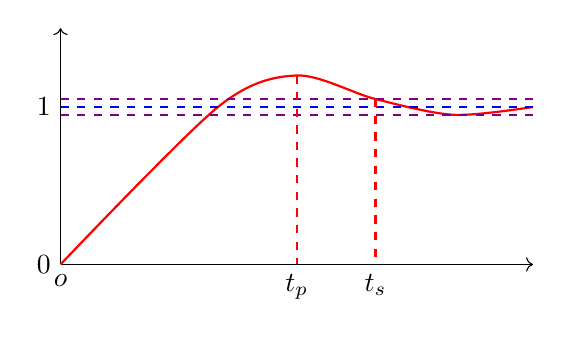
\begin{tikzpicture}[scale=2]
\coordinate (o) at (0,0);
\coordinate (ox) at (3,0);
\coordinate (oy) at (0,1.5);
\draw[->] (o) -- (ox);
\draw[->] (o) -- (oy);
\draw (o) node[below] {$o$};
\draw [red,thick,smooth] plot coordinates {(0,0) (1,1) (1.5,1.2) (2,1.05) (2.5,0.95) (3,1)};
\draw[thick,blue,dashed] (0,1) -- (3,1);
\draw[thick,violet,dashed] (0,0.95) -- (3,0.95);
\draw[thick,violet,dashed] (0,1.05) -- (3,1.05);
\draw[thick,red,dashed] (1.5,1.2) -- (1.5,0);\draw (1.5,0) node[below] {$t_p$};
\draw[thick,red,dashed] (2,1.05) -- (2,0);\draw (2,0) node[below] {$t_s$};
\draw (o) node[left] {$0$}
;\draw (0,1) node[left] {$1$};
\end{tikzpicture}


\item 指标:\\
\label{sec-3-2-2-2}%
\begin{itemize}
\item <2->超调量 $\sigma\%$
\item <3->调节时间 $t_s$
\item <4->上升时间 $t_r$
\end{itemize}
\begin{itemize}
\item <5->峰值时间 $t_p$
\end{itemize}

\end{itemize} % ends low level
\end{frame}
\begin{frame}
\frametitle{指标}
\label{sec-3-2-3}

\begin{itemize}
\item 超调量:  $(c(t_p)-c(\infty))/c(\infty)$
\item 调节时间: 若有 $t_s$ ,当 $t\geq t_s$ 时有 $|c(t)-c(\infty)|\leq 0.05c(\infty)$ (或 $0.03c(\infty)$ )成立,则 $t_s$ 为该系统调节时间。
\item 上升时间 $t_r$ ,定义
\begin{itemize}
\item $100\%$ 的 $t_r,c(t)$ 首次达到 $c(\infty)$ 的时间
\item $90\%$ 的 $t_r,c(t)$ 首次达到 $90\%c(\infty)$ 的时间
\item $70\%$ 的 $t_r,c(t)$ 首次达到 $70\%c(\infty)$ 的时间
\end{itemize}
\item 峰值时间 $t_p$ : $c(t_p)=Max(c(t))$
\end{itemize}
\end{frame}

\end{document}
